\uuid{soNU}
\exo7id{5425}
\titre{exo7 5425}
\auteur{rouget}
\organisation{exo7}
\datecreate{2010-07-06}
\isIndication{false}
\isCorrection{true}
\chapitre{Suite}
\sousChapitre{Suite définie par une relation de récurrence}
\module{Analyse}
\niveau{L1}
\difficulte{}

\contenu{
\texte{
Etudier la suite $(u_n)$ dans chacun des cas suivants~:

$$\begin{array}{ll}
1)\;u_0\geq-1\;\mbox{et}\;\forall n\in\Nn,\;u_{n+1}=\sqrt{1+u_n},&2)\;u_0>-1\;\mbox{et}\;\forall n\in\Nn,\;u_{n+1}=\ln(1+u_n)\\
3)\;u_0\in\Rr\;\mbox{et}\;\forall n\in\Nn,\;u_{n+1}=\sin u_n,&4)\;u_0\in\Rr\;\mbox{et}\;\forall n\in\Nn,\;u_{n+1}=\cos(u_n),\\
5)\;u_0\in\Rr\;\mbox{et}\;\forall n\in\Nn,\;u_{n+1}=\sin(2u_n),&6)\;u_0\in\Rr\;\mbox{et}\;\forall n\in\Nn,\;u_{n+1}=u_n^2-2u_n+2.
\end{array}
$$
}
\reponse{
Pour $x\geq-1$, posons $f(x)=\sqrt{1+x}$ et $g(x)=f(x)-x$.

Soit $u_0\in I=[-1,+\infty[$. $f$ est définie sur $I$ et de plus $f(I)=[0,+\infty[\subset[-1,+\infty[$. On en déduit, par une démonstration par récurrence, que la suite $u$ est définie.

Si la suite $u$ converge, puisque $\forall n\in\Nn,\;u_n\geq-1$, sa limite $\ell$ vérifie $\ell\geq-1$. Puisque $f$ est continue sur $[-1,+\infty[$ et donc en $\ell$,

$$\ell=\lim_{n\rightarrow +\infty}u_{n+1}=\lim_{n\rightarrow +\infty}f(u_n)=f(\lim_{n\rightarrow +\infty}u_n)=f(ell).$$

et $\ell$ est un point fixe de $f$. Or, pour $x\geq-1$,

\begin{align*}\ensuremath
\sqrt{1+x}=x&\Leftrightarrow1+x=x^2\;\mbox{et}\;x\geq0\Leftrightarrow(x=\frac{1-\sqrt{5}}{2}\;\mbox{ou}\;x=\frac{1+\sqrt{5}}{2})\;
\mbox{et}\;x\geq0\\
 &\Leftrightarrow x=\frac{\sqrt{5}+1}{2}.
\end{align*}

Ainsi, si la suite $(u_n)$ converge, c'est vers le nombre $\alpha=\frac{\sqrt{5}+1}{2}$.

Pour $x\geq-1$,

\begin{align*}\ensuremath
\mbox{sgn}(f(x)-\alpha)&=\mbox{sgn}(\sqrt{1+x}-\sqrt{1+\alpha})=\mbox{sgn}((1+x)-(1+\alpha))\quad(\mbox{par croissance de}\;x\mapsto x^2\;\mbox{sur}\;[0,+\infty[)\\
 &=\mbox{sgn}(x-\alpha).
\end{align*}

Ainsi, les intervalles $[-1,\alpha[$ et $]\alpha,+\infty[$ sont stables par $f$. Donc, si $-1\leq u_0<\alpha$, alors par récurrence $\forall n\in\Nn,\;-1\leq u_n<\alpha$ et si $u_0>\alpha$, alors par récurrence, $\forall n\in\Nn,\;u_n>\alpha$.

Soit $x\geq-1$. Si $x\in[-1,0]$, $\sqrt{1+x}-x\geq0$ et si $x\geq0$,

\begin{align*}\ensuremath
\mbox{sgn}(g(x))&=\mbox{sgn}(\sqrt{1+x}-x)\\
 &=\mbox{sgn}((1+x)-x^2)\quad(\mbox{par croissance de}\;x\mapsto x^2\;\mbox{sur}\;[0,+\infty[)\\
 &=\mbox{sgn}(x+\frac{\sqrt{5}-1}{2})(-x+\frac{1+\sqrt{5}}{2}-x)=\mbox{sgn}(\alpha-x)\;(\mbox{car ici}\;x\geq0).
\end{align*}

On en déduit que, si $x\in[-1,\alpha[$, $f(x)>x$, et si $x\in]\alpha,+\infty[$, $f(x)<x$. Mais alors, 
si $-1\leq u_0<\alpha$, puisque $\forall n\in\Nn,\;-1\leq u_n<\alpha$, pour $n$ entier naturel donné, on a

$$u_{n+1}=f(u_n)>u_n.$$

La suite $u$ est donc strictement croissante, majorée par $\alpha$ et donc convergente. On sait de plus que sa limite est nécessairement $\alpha$.

Si $u_0>\alpha$, puisque $\forall n\in\Nn,\;u_n>\alpha$, pour $n$ entier naturel donné, on a

$$u_{n+1}=f(u_n)<u_n.$$

La suite $u$ est donc strictement décroissante, minorée par $\alpha$ et donc convergente. On sait de plus que sa limite est nécessairement $\alpha$. Enfin, si $u_0=\alpha$, la suite $u$ est constante.

En résumé,

si $u_0\in[-1,\frac{\sqrt{5}+1}{2}[$, la suite $u$ est strictement croissante, convergente de limite $\frac{\sqrt{5}+1}{2}[$,

si $u_0\in]\frac{\sqrt{5}+1}{2},+\infty[$, la suite $u$ est strictement décroissante, convergente de limite $\frac{\sqrt{5}+1}{2}[$,

si $u_0=\frac{\sqrt{5}+1}{2}[$, la suite $u$ est constante et en particulier convergente de limite $\frac{\sqrt{5}+1}{2}$.

Ainsi, dans tous les cas, la suite $u$ est convergente et $\lim_{n\rightarrow +\infty}u_n=\frac{1+\sqrt{5}}{2}$.

$$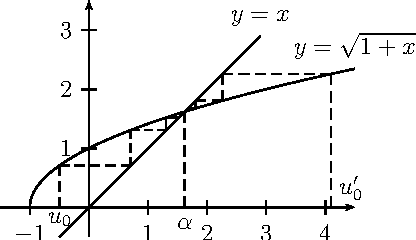
\includegraphics{../images/pdf/soNU-1.pdf}$$
Si $u_0>0$, alors puisque $f$ est définie sur l'intervalle $I=]0,+\infty[$ et que $I$ est stable par $f$ ($\forall x>0,\;\ln(1+x)>\ln1=0$), la suite $u$ est définie et est strictement positive. Si la suite $u$ converge, sa limite $\ell$ est un réel positif \textbf{ou nul}. Par continuité de $f$ sur $[0,+\infty[$ et donc en $\ell$,

$$\ell=\lim_{n\rightarrow +\infty}u_{n+1}=\lim_{n\rightarrow +\infty}f(u_n)=f(\lim_{n\rightarrow +\infty}u_n)=f(\ell).$$

Pour $x>-1$, posons $g(x)=\ln(1+x)-x$. $g$ est définie et dérivable sur $]-1,+\infty[$ et pour $x>-1$,

$$g'(x)=\frac{1}{1+x}-1=-\frac{x}{1+x}.$$

$g'$ est strictement positive sur $]-1,0[$ et strictement négative sur $]0,+\infty[$. $g$ est donc strictement croissante sur $]-1,0]$ et strictement décroissante sur $[0,+\infty[$. Par suite, si $x\in]-1,0[\cup]0,+\infty[$, $g(x)<0$. En particulier, pour $x\in]-1,0[\cup]0,+\infty[$, $f(x)\neq x$. Puisque $f(0)=0$, $f$ admet dans $]-1,+\infty[$ un et un seul point fixe à savoir $0$.

En résumé, si $u_0>0$, la suite $u$ est définie, strictement positive, et de plus, si la suite $u$ converge, alors $\lim_{n\rightarrow +\infty}u_n=0$.

Mais, pour $n$ entier naturel donné,

$$u_{n+1}-u_n=\ln(1+u_n)-u_n<0.$$

Par suite, la suite $u$ est strictement décroissante, minorée par $0$ et donc, d'après ce qui précède, converge vers $0$.

Si $u_0=0$, la suite $u$ est constante. Il reste donc à étudier le cas où $u_0\in]-1,0[$. Montrons par l'absurde qu'il existe un rang $n_0$ tel que $u_{n_0}\leq-1$. Dans le cas contraire, $\forall n\in\Nn,\;u_n>-1$. Comme précédemment, par récurrence, la suite $u$ est à valeurs dans $]-1,0[$ et strictement décroissante. Etant minorée par $-1$, la suite $u$ converge vers un certain réel $\ell$.

Puisque $\forall n\in\Nn,\;-1<u_n\leq u_0<0$, on a $-1\leq\ell\leq u_0<0$. Donc, ou bien $\ell=-1$, ou bien $f$ est continue en $\ell$ et $\ell$ est un point fixe de $f$ élément de $]-1,0[$.

On a vu que $f$ n'admet pas de point fixe dans $]-1,0[$ et donc ce dernier cas est exclu. Ensuite, si $\ell=-1$, il existe un rang $N$ tel que $u_N\leq -0.9$. Mais alors, $u_{N+1}=\leq\ln(-0,9+1)=-2,3...<-1$ ce qui constitue de nouveau une contradiction.

Donc, il existe un rang $n_0$ tel que $u_{n_0}\leq-1$ et la suite $u$ n'est pas définie à partir d'un certain rang.

En résumé,

si $u_0\in]0,+\infty[$, la suite $u$ est strictement décroissante, convergente et $\lim_{n\rightarrow +\infty}u_n=0$,

si $u_0=0$, la suite $u$ est constante,

et si $u_0\in]-1,0[$, la suite $u$ n'est pas définie à partir d'un certain rang.

$$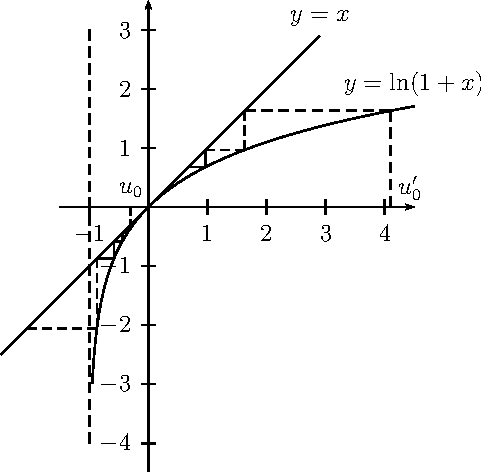
\includegraphics{../images/pdf/soNU-2.pdf}$$
Pour tout choix de $u_0$, $u_1\in[-1,1]$. On supposera dorénavant que $u_0\in[-1,1]$. Si $u_0=0$, la suite $u$ est constante. Si $u_0\in[-1,0[$, considérons la suite $u'$ définie par $u_0'=-u_0$ et $\forall n\in\Nn,\;u_{n+1}'=\sin(u_n')$. La fonction $x\mapsto\sin x$, il est clair par récurrence que $\forall n\in\Nn,\;u_n'=-u_n$. On supposera dorénavant que $u_0\in]0,1]$.

Puisque $]0,1]\subset]0,\frac{\pi}{2}]$, on a $\sin]0,1]\subset]0,1]$ et l'intervalle $I=]0,1]$ est stable par $f$. Ainsi, si $u_0\in]0,1]$, alors, $\forall n\in\Nn,\;u_n\in]0,1]$.

Pour $x\in[0,1]$, posons $g(x)=\sin x-x$. $g$ est dérivable sur $[0,1]$ et pour $x\in[0,1]$, $g'(x)=\cos x-1$. $g'$ est strictement négative sur $]0,1]$ et donc strictement décroissante sur $[0,1]$. On en déduit que pour $x\in]0,1]$, $g(x)<g(0)=0$.

Mais alors, pour $n$ entier naturel donné, $u_{n+1}=\sin(u_n)<u_n$. La suite $u$ est ainsi strictement décroissante, minorée par $0$ et donc converge vers $\ell\in[0,1]$. La fonction $x\mapsto\sin x$ est continue sur $[0,1]$ et donc, $\ell$ est un point fixe de $f$. L'étude de $g$ montre que $f$ a un et un seul point fixe dans $[0,1]$ à savoir $0$. La suite $u$ est donc convergente et $\lim_{n\rightarrow +\infty}u_n=0$.

L'étude préliminaire montre la suite $u$ converge vers $0$ pour tout choix de $u_0$.

$$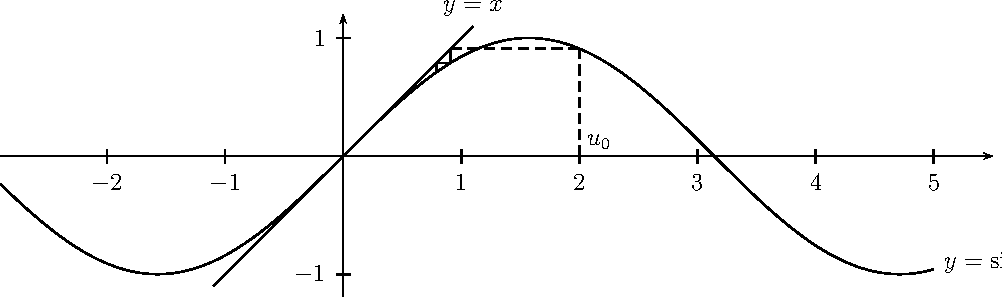
\includegraphics{../images/pdf/soNU-3.pdf}$$
Si $u_0$ est un réel quelconque, $u_1\in[-1,1]\subset[-\frac{\pi}{2},\frac{\pi}{2}]$ puis $u_2\in[0,1]$. On supposera dorénavant que $u_0\in[0,1]$.

On a $\cos([0,1])=[\cos 1,\cos0]=[0,504...,1]\subset[0,1]$. Donc, la fonction $x\mapsto\cos x$ laisse stable l'intervalle $I=[0,1]$. On en déduit que $\forall n\in\Nn,\;u_n\in[0,1]$.

Pour $x\in[0,1]$, on pose $g(x)=\cos x-x$. $g$ est somme de deux focntions strictement décroissantes sur $[0,1]$ et est donc strictement décroissante sur $[0,1]$. De plus, $g$ est continue sur $[0,1]$ et vérifie $g(0)=\cos0>0$ et $g(1)=\cos1-1<0$. $g$ s'annule donc une et une seule fois sur $[0,1]$ en un certain réel $\alpha$. Ainsi, $f$ admet sur $[0,1]$ un unique point fixe, à savoir $\alpha$. Puisque $f$ est continue sur le segment $[0,1]$, on sait que si la suite $u$ converge, c'est vers $\alpha$.

La fonction $f~:~x\mapsto\cos x$ est dérivable sur $[0,1]$ et pour $x\in[0,1]$,

$$|f'(x)|=|-\sin x|\leq\sin1<1.$$

L'inégalité des accroissements finis montre alors que $\forall(x,y)\in[0,1]^2,\;|\cos x-\cos y|\leq\sin1|x-y|$. Pour $n$ entier naturel donné, on a alors

$$|u_{n+1}-\alpha|=|f(u_n)-f(\alpha)|\leq\sin1|u_n-\alpha|,$$

et donc, pour tout entier naturel $n$,

$$|u_n-\alpha|\leq(\sin1)^n|u_0-\alpha|\leq(\sin1)^n.$$

Comme $0\leq\sin1<1$, la suite $(\sin1)^n$ converge vers $0$, et donc la suite $(u_n)_{n\in\Nn}$ converge vers $\alpha$. On peut noter que puisque la fonction $x\mapsto\cos x$ est strictement décroissante sur $[0,1]$, les deux suites $(u_{2n})_{n\in\Nn}$ et $(u_{2n+1})_{n\in\Nn}$ sont strictement monotones, de sens de variations contraires (dans le cas où $u_0\in[0,1]$. On peut noter également que si $n>\frac{\ln(10^{-2})}{\ln(\sin1)}=26,6...$, alors $(\sin1)^n<10^{-2}$. Par suite, $u_{27}$ est une valeur approchée de $\alpha$ à $10^{-2}$ près. La machine fournit $\alpha=0,73...$ (et même $\alpha=0,739087042.....$).

$$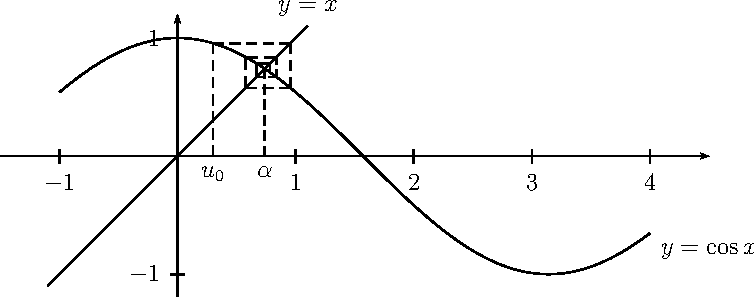
\includegraphics{../images/pdf/soNU-4.pdf}$$
Si $u_0$ est un réel quelconque, alors $\forall n\in\Nn^*,\;u_n\in[-1,1]$. On supposera sans perte de généralité que $u_0\in[-1,1]$. Si $u_0=0$, la suite $u$ est constante et d'autre part, l'étude du cas $u_0\in[-1,0[$ se ramème, comme en 3), à l'étude du cas $u_0\in]0,1]$. On supposera dorénavant que $u_0\in]0,1]$.

Si $x\in]0,1]$, alors $2x\in]0,2]\subset]0,\pi[$ et donc $\sin(2x)\in]0,1]$. L'intervalle $I=]0,1]$ est donc stable par la fonction $f~:~x\mapsto\sin(2x)$. On en déduit que $\forall n\in\Nn,\;u_n\in]0,1]$.

Pour $x\in[0,1]$, posons $g(x)=\sin(2x)-x$. $g$ est dérivable sur $[0,1]$ et pour $x\in[0,1]$, $g'(x)=2\cos(2x)-1$. $g$ est donc strictement croissante sur $[0,\frac{\pi}{4}]$ et strictement décroissante sur $[\frac{\pi}{4},1]$. On en déduit que si $x\in]0,\frac{\pi}{4}]$, $g(x)>g(0)=0$. D'autre part, $g$ est continue et strictement décroissante sur $[\frac{\pi}{4},1]$ et vérifie $g(\frac{\pi}{4})=1-\frac{\pi}{4}>0$ et $g(1)=\sin2-1<0$. $g$ s'annule donc une et une seule fois en un certain réel $\alpha\in]\frac{\pi}{4},1[$.

En résumé, $g$ s'annule une et une seule fois sur $]0,1]$ en un certain réel $\alpha\in]\frac{\pi}{4},1[$, $g$ est strictement positive sur $]0,\alpha[$ et strictement négative sur $]\alpha,1]$.

Supposons que $u_0\in]0,\frac{\pi}{4}[$ et montrons par l'absurde que $\exists n_0\in\Nn/\;u_{n_0}\in[\frac{\pi}{4},1]$. Dans le cas contraire, tous les $u_n$ sont dans $]0,\frac{\pi}{4}[$. Mais alors, pour tout entier naturel $n$,

$$u_{n+1}-u_n=f(u_n)-u_n=g(u_n)>0.$$

La suite $u$ est donc strictement croissante. Etant majorée par $\frac{\pi}{4}$, la suite $u$ converge. Comme $g$ est continue sur $[u_0,\frac{\pi}{4}]$ et que $\forall n\in\Nn,\;u_n\in[u_0,\frac{\pi}{4}]$, on sait que la limite de $u$ est un point fixe de $f$ élément de $[u_0,\frac{\pi}{4}]$. Mais l'étude de $g$ a montré que $f$ n'admet pas de point fixe dans cet intervalle ($u_0$ étant strictement positif). On aboutit à une contradiction.

Donc, ou bien $u_0\in[\frac{\pi}{4},1]$, ou bien $u_0\in]0,\frac{\pi}{4}[$ et dans ce cas, $\exists n_0\in\Nn/\;u_{n_0}\in[\frac{\pi}{4},1]$. Dans tous les cas, $\exists n_0\in\Nn/\;u_{n_0}\in[\frac{\pi}{4},1]$. Mais alors, puisque $f([\frac{\pi}{4},1])=[\sin2,\sin\frac{\pi}{2}]\subset[\frac{\pi}{4},1]$ (car $\sin2=0,909...>0,785...=\frac{\pi}{4}$), pour tout entier $n\geq n_0$, $u_n\in[\frac{\pi}{4},1]$.

Pour $x\in[\frac{\pi}{4},1]$, $|g'(x)|=|2\cos(2x)|\leq|2\cos2|$. L'inégalité des accroissements finis montre alors que $\forall n\geq n_0,\;|u_{n+1}-\alpha|\leq|2\cos2|.|u_n-\alpha|$, puis que 

$$\forall n\geq n_0,\;|u_n-\alpha|\leq|2\cos2|^{n-n_0}|u_{n_0}-\alpha|.$$

Comme $|2\cos2|=0,83...<1$, on en déduit que la suite $u$ converge vers $\alpha$. La machine donne par ailleurs $\alpha=0,947...$.

$$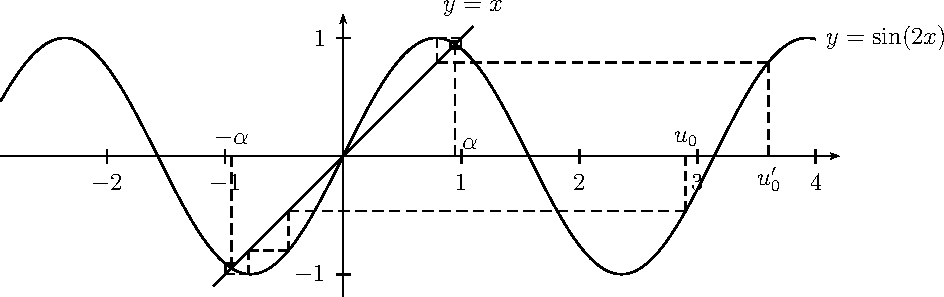
\includegraphics{../images/pdf/soNU-5.pdf}$$
Pour $x\in\Rr$,

$$x^2-2x+2=x\Leftrightarrow x^2-3x+2=0\Leftrightarrow(x-1)(x-2)=0\Leftrightarrow x=1\;\mbox{ou}\;x=2.$$

Donc, si la suite $u$ converge, ce ne peut être que vers $1$ ou $2$.

Pour $n\in\Nn$,

$$\begin{array}{l}
u_{n+1}-u_n=(u_n^2-2u_n+2)-u_n=(u_n-1)(u_n-2)\quad(I)\\
u_{n+1}-1=u_n^2-2u_n+1=(u_n-1)^2\quad(II)\\
u_{n+1}-2=u_n^2-2u_n=u_n(u_n-2)\quad(III).
\end{array}
$$

\begin{itemize}
[\textbf{1er cas.}] Si $u_0=1$ ou $u_0=2$, la suite $u$ est constante.
[\textbf{2ème cas.}] Si $u_0\in]1,2[$, $(II)$ et $(III)$ permettent de montrer par récurrence que $\forall n\in\Nn,\;u_n\in]1,2[$. $(I)$ montre alors que la suite $u$ est strictement décroissante. Etant minorée par $1$, elle converge vers un réel $\ell\in[1,u_0]\subset[1,2[$. Dans ce cas, la suite $(u_n)$ converge vers $1$.
[\textbf{3ème cas.}] Si $u_0\in]2,+\infty[$, $(III)$ permet de montrer par récurrence que $\forall n\in\Nn,\;u_n>2$. Mais alors, $(I)$ montre que la suite $u$ est strictement croissante. Si $u$ converge, c'est vers un réel $\ell\in[u_0,+\infty[\subset]2,+\infty[$. $f$ n'ayant pas de point fixe dans cet intervalle, la suite $u$ diverge et, $u$ étant strictement croissante, on a $\lim_{n\rightarrow +\infty}u_n=+\infty$.
[\textbf{4ème cas.}] Si $u_0\in]0,1[$, alors $u_1=(u_0-1)^2+1\in]1,2[$ ce qui ramène au deuxième cas. La suite $u$ converge vers $1$.
[\textbf{5ème cas.}] Si $u_0=0$, alors $u_1=2$ et la suite $u$ est constante à partir du rang $1$. Dans ce cas, la suite $u$ converge vers $2$.
[\textbf{6ème cas.}] Si $u_0<0$, alors $u_1=u_n^2-2u_n+2>2$, ce qui ramène au troisième cas. La suite $u$ tend vers $+\infty$.
\end{itemize}

En résumé, si $u_0\in]0,2[$, la suite $u$ converge vers $1$, si $u_0\in\{0,2\}$, la suite $u$ converge vers $2$ et si $u_0\in]-\infty,0[\cup]2,+\infty[$, la suite $u$ tend vers $+\infty$.

$$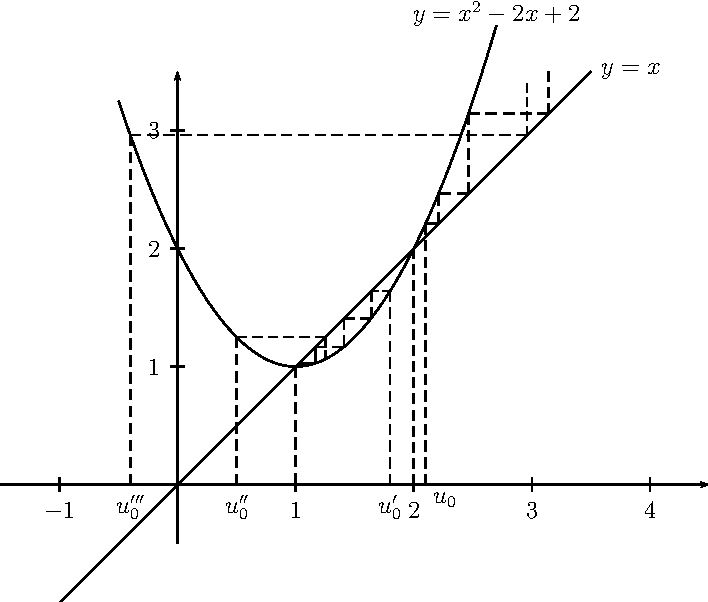
\includegraphics{../images/pdf/soNU-6.pdf}$$
}
}
